\section{Preliminaries}

\begin{frame}{Graph Neural Networks (GNNs)}

    Supervised ML: $\quad \mathcal{D} \coloneqq \set{(\xx_i, \yy_i)}_{i=1}^n$, $\xx_i \in \R^{d}$, $\yy_i \in \R^k$, with $\xx_i$ \textbf{iid}

    \begin{figure}[H]
        \begin{subfigure}[t]{0.3\textwidth}
            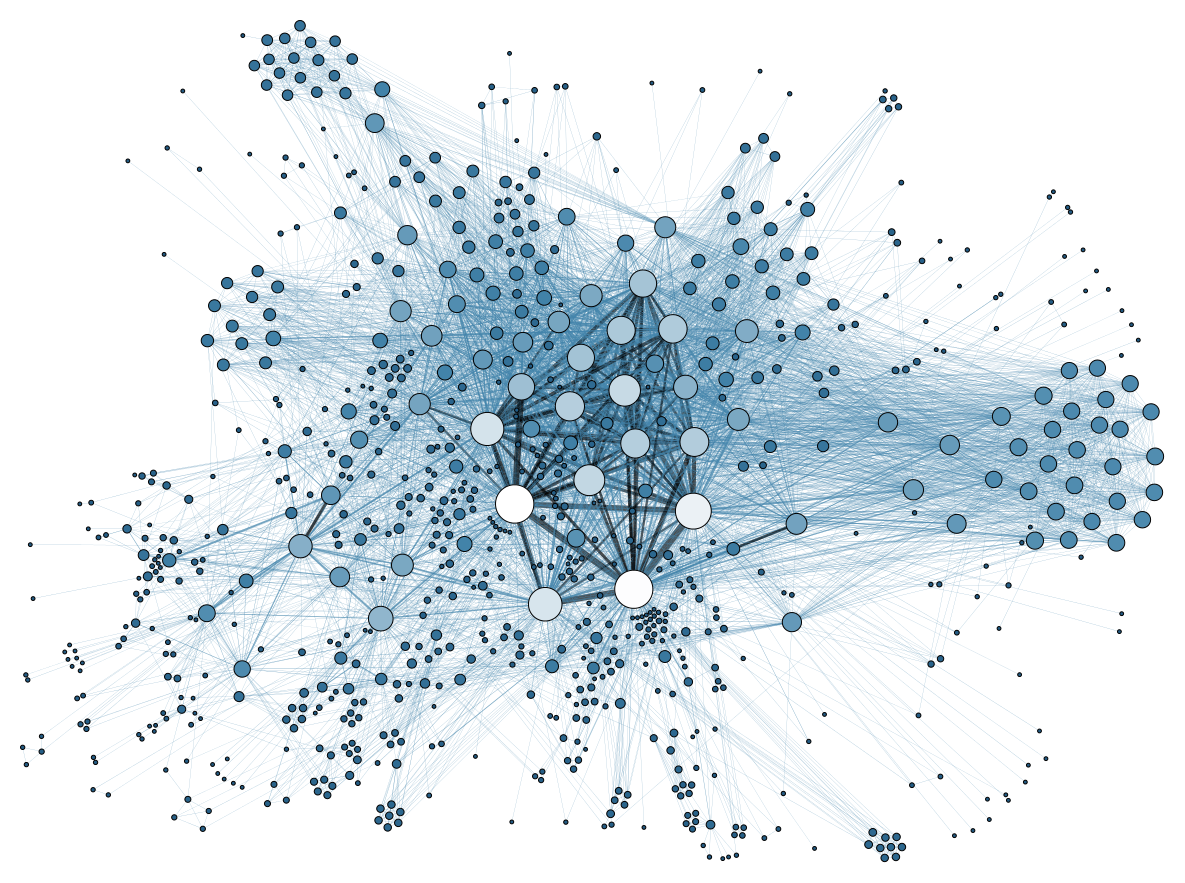
\includegraphics[width=\textwidth]{figures/gnns/social_network.png}
        \end{subfigure} \hspace*{1em}%
        ~
        \begin{subfigure}[t]{0.3\textwidth}
            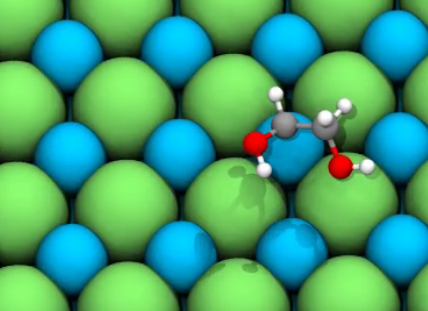
\includegraphics[width=\textwidth]{figures/gnns/molecule.png}
        \end{subfigure}
        \vspace*{-1em}
    \end{figure}

    $\rightarrow$ What if our data looks like this?\footfullcite{social_network}\footfullcite{molecule}
\end{frame}

\begin{frame}{Graph Networks (GNs)\footfullcite{https://doi.org/10.48550/arxiv.1806.01261}}

    Graph $G$ with nodes $V$, edges $E$ and global attribute $\uu$:
    \[
        G \: = \: (\uu, V, E) \text{,} \quad \uu \in \R^{d_u} \text{;}
    \]
    node embeddings $\vv_i$ and edge embeddings $\ee_i$:
    \begin{align*}
        V \: &= \: \set{\vv_i}_{i=1}^{n_v},             &\quad \vv_i \in \R^{d_v}&; \\
        E \: &= \: \set{(\ee_k, r_k, s_k)}_{k=1}^{n_e}, &\quad \ee_k \in \R^{d_e}&, \; r_k, s_k \in \set{1, \dots, n_v};
    \end{align*}
    
\end{frame}

\begin{frame}{GN block}
    
    \begin{align*}
        &\text{Update} & & \text{Aggregation} \\
        \vspace*{2em}
        \ee_k' \: &\coloneqq \: \phi_e(\ee_k, \vv_{r_k}, \vv_{s_k}, \uu), 
        &\overline{\ee}'_i \: &\coloneqq \: \rho_{e \to v}(E_i'), \\
        \vv_i' \: &\coloneqq \: \phi_v(\overline{\ee}'_i, \vv_i, \uu), 
        &\overline{\ee}' \: &\coloneqq \: \rho_{e \to u}(E'), \\
        \uu' \: &\coloneqq \: \phi_u(\overline{\ee}', \overline{\vv}', \uu),
        &\overline{\vv}' \: &\coloneqq \: \rho_{v \to u}(V');
    \end{align*}

    \begin{figure}[H]
    \centering
    \tikzset{
        n_inactive/.style={draw=tum-gray, fill=white, text=tum-gray, circle},
        n_active/.style={draw=tum-gray, fill=tum-lighter-blue, text=tum-dark-blue, circle},
        n_updated/.style={draw=tum-gray, fill=tum-light-orange, text=tum-orange, circle},
        e_inactive/.style={draw=tum-gray},
        e_active/.style={draw=tum-blue, thick},
        e_updated/.style={draw=tum-orange, thick}
    }

    \makeatletter
    \tikzset{circle split part fill/.style  args={#1,#2}{%
    alias=tmp@name,
    postaction={%
        insert path={
        \pgfextra{% 
        \pgfpointdiff{\pgfpointanchor{\pgf@node@name}{center}}%
                    {\pgfpointanchor{\pgf@node@name}{east}}%            
        \pgfmathsetmacro\insiderad{\pgf@x}
        \fill[#1] (\pgf@node@name.base) ([xshift=-\pgflinewidth]\pgf@node@name.east) arc
                            (0:180:\insiderad-\pgflinewidth)--cycle;
        \fill[#2] (\pgf@node@name.base) ([xshift=\pgflinewidth]\pgf@node@name.west)  arc
                            (180:360:\insiderad-\pgflinewidth)--cycle;   
            }}}}}  
 \makeatother

    \begin{subfigure}[t]{0.16\textwidth}
        \centering
        \begin{tikzpicture}[scale=0.81]
            % Edge Update
            \draw[rounded corners] (-0.6,-1.5) rectangle (2,1.5) {};
            \node[text=tum-dark-blue] (T) at (1.65,1.2) {\tiny $\uu$};
    
            \node[n_active, inner sep=1] (A) at (1,0) {\tiny $\vv_{r_k}$};
            \node[n_active, inner sep=1] (B) at (0,0.6) {\tiny $\vv_{s_k}$};
            \node[n_inactive] (C) at (0.3,-0.7) {};
            \node[n_inactive] (D) at (1.4, -1) {};
    
            \draw[->, e_updated] (B) -- (A) node[text=tum-orange, near end, above] {\tiny $\ee_k'$};
            \draw[->, e_inactive] (C) -- (A);
            \draw[->, e_inactive] (D) -- (A);
            \draw[<->, e_inactive] (C) -- (D);
        \end{tikzpicture}
        \caption*{\scriptsize Edge Update}
    \end{subfigure}%
    ~
    \begin{subfigure}[t]{0.3\textwidth}
        \centering
        \begin{tikzpicture}[scale=0.81]
            %Edge Aggregation
            \draw[rounded corners] (-0.6,-1.5) rectangle (4.6,1.5) {};
            \draw[] (2,-1.5) -- (2,1.5);
            \node[text=tum-gray] (T) at (1.65,1.2) {\tiny $\uu$};
    
            \node[n_inactive, inner sep=1, circle split, circle split part fill={white,tum-light-orange}] (A) at (1,0) {\tiny $\vv_i$ \nodepart{lower} \textcolor{tum-orange}{\tiny $\overline{\ee}_i'$}};
            \node[n_inactive] (B) at (0,0.6) {};
            \node[n_inactive] (C) at (0.3,-0.7) {};
            \node[n_inactive] (D) at (1.4, -1) {};
    
            \draw[->, e_active] (B) -- (A);
            \draw[->, e_active] (C) -- (A);
            \draw[->, e_active] (D) -- (A);
            \draw[<->, e_inactive] (C) -- (D);

            \begin{scope}[shift={(2.6, 3.5)}]
                \node[text=tum-gray] (T) at (1.65,-2.3) {\tiny $\uu$};
                \node[text=tum-orange] (T) at (1.7,-2.6) {\tiny $\overline{\ee}'$};
        
                \node[n_inactive] (A) at (1,-3.5) {};
                \node[n_inactive] (B) at (0,-2.9) {};
                \node[n_inactive] (C) at (0.3,-4.2) {};
                \node[n_inactive] (D) at (1.4, -4.5) {};
        
                \draw[->, e_active] (B) -- (A);
                \draw[->, e_active] (C) -- (A);
                \draw[->, e_active] (D) -- (A);
                \draw[<->, e_active] (C) -- (D);
            \end{scope}
        \end{tikzpicture}
        \caption*{\scriptsize Edge Aggr.}
    \end{subfigure}%
    ~
    \begin{subfigure}[t]{0.16\textwidth}
        \centering
        \begin{tikzpicture}[scale=0.81]
            % Node Update
            \draw[rounded corners] (-0.6,-1.5) rectangle (2,1.5) {};
            \node[text=tum-dark-blue] (T) at (1.65,1.2) {\tiny $\uu$};
            \node[text=tum-gray] (T) at (1.7,0.9) {\tiny $\overline{\ee}'$};
    
            \node[n_inactive, inner sep=1, circle split, circle split part fill={tum-light-orange,tum-lighter-blue}] (A) at (1,0) {\tiny \textcolor{tum-orange}{$\vv_i'$} \nodepart{lower} \textcolor{tum-dark-blue}{\tiny $\overline{\ee}_i'$}};
            \node[n_inactive] (B) at (0,0.6) {};
            \node[n_inactive] (C) at (0.3,-0.7) {};
            \node[n_inactive] (D) at (1.4, -1) {};
    
            \draw[->, e_inactive] (B) -- (A);
            \draw[->, e_inactive] (C) -- (A);
            \draw[->, e_inactive] (D) -- (A);
            \draw[<->, e_inactive] (C) -- (D);
        \end{tikzpicture}
        \caption*{\scriptsize Node Update}
    \end{subfigure}%
    ~
    \begin{subfigure}[t]{0.16\textwidth}
        \centering
        \begin{tikzpicture}[scale=0.81]
            % Node Aggregation
            \draw[rounded corners] (-0.6,-1.5) rectangle (2,1.5) {};
            \node[text=tum-gray] (T) at (1.65,1.2) {\tiny $\uu$};
            \node[text=tum-gray] (T) at (1.7,0.9) {\tiny $\overline{\ee}'$};
            \node[text=tum-orange] (T) at (1.7,0.6) {\tiny $\overline{\vv}'$};

            \node[n_active] (A) at (1,0) {};
            \node[n_active] (B) at (0,0.6) {};
            \node[n_active] (C) at (0.3,-0.7) {};
            \node[n_active] (D) at (1.4, -1) {};
    
            \draw[->, e_inactive] (B) -- (A);
            \draw[->, e_inactive] (C) -- (A);
            \draw[->, e_inactive] (D) -- (A);
            \draw[<->, e_inactive] (C) -- (D);
        \end{tikzpicture}
        \caption*{\scriptsize Node Aggr.}
    \end{subfigure}%
    ~
    \begin{subfigure}[t]{0.16\textwidth}
        \centering
        \begin{tikzpicture}[scale=0.81]
            %Global Update
            \draw[rounded corners] (-0.6,-1.5) rectangle (2,1.5) {};
            \node[text=tum-orange] (T) at (1.7,1.2) {\tiny $\uu'$};
            \node[text=tum-dark-blue] (T) at (1.7,0.9) {\tiny $\overline{\ee}'$};
            \node[text=tum-dark-blue] (T) at (1.7,0.6) {\tiny $\overline{\vv}'$};


            \node[n_inactive] (A) at (1,0) {};
            \node[n_inactive] (B) at (0,0.6) {};
            \node[n_inactive] (C) at (0.3,-0.7) {};
            \node[n_inactive] (D) at (1.4, -1) {};
    
            \draw[->, e_inactive] (B) -- (A);
            \draw[->, e_inactive] (C) -- (A);
            \draw[->, e_inactive] (D) -- (A);
            \draw[<->, e_inactive] (C) -- (D);
        \end{tikzpicture}
        \caption*{\scriptsize Global Update}
    \end{subfigure}

\end{figure}

\end{frame}

\begin{frame}{Extended Graph Networks (EGNs) \footfullcite{https://doi.org/10.48550/arxiv.2203.09697}}
    Graph
    \[ G \: \coloneqq \: (\uu, V, E, T) \]
    with higher-order interactions
    \[
        T \: \coloneqq \: \set{(\ttt_m, e_1^{(m)}, \dots, e_{l_m}^{(m)})}_{m=1}^{n_t}, 
        \qquad \ttt_m \in \R^{d_t} \text{.}
    \]
\end{frame}

\begin{frame}{GNNs for atomic simulations}

    \begin{itemize}
        \bitem Want to predict properties of molecules: energy and forces
        \bitem Traditional method: Density Functional Theory $\rightarrow$ very slow!
    \end{itemize}
    $\Rightarrow$ Use GNNs for this!

    \begin{itemize}
        \bitem Molecule consists of atomic numbers $\zz$ and positions $\XX$:
        \[
            \XX \: \coloneqq \: \set{\xx_1, \dots, \xx_n}, \; \xx_i \in \R^3
            \quad \text{and} \quad 
            \zz \: \coloneqq \: \set{z_1, \dots, z_n}, \; z_i \in \N \text{.}
            \label{eq:molecule_setup}
        \]
    \end{itemize}
    $\Rightarrow$ lots of invariances!
    
\end{frame}

\begin{frame}{GNNs for atomic simulations}
    Only use distances $d_{ij} = \norm{\xx_i - \xx_j}_2$?
    \begin{figure}[H]
        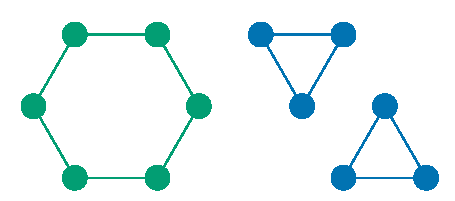
\includegraphics[width=0.4\textwidth]{figures/gnns/indistinguishable.pdf}
        \vspace*{-1em}
    \end{figure}
    \begin{center}
        $\;\Rightarrow\;$ \textbf{problem!}\footfullcite{DBLP:journals/corr/abs-2003-03123}
    \end{center}

    $\Rightarrow$ Solution: Take bond angles (triplets of nodes) into account.

\end{frame}

\begin{frame}{Force-centric vs. energy-centric models}
    Observation: 
    \[
        \FF_i \: \coloneqq \: \frac{\partial E(\XX, \zz)}{\partial \xx_i} \: \in \: \R^3.
    \]
    \begin{columns}
        \centering
        \begin{column}{0.35\textwidth}
           \begin{center}
                \textbf{Force-centric}
           \end{center}
           Predict molecule energy and per-atom forces directly. \textcolor{black!2}{filler}
        \end{column}
        \begin{column}{0.15\textwidth}
            \begin{center}
                $\boldsymbol{\leftrightarrow}$
            \end{center}
        \end{column}
        \begin{column}{0.35\textwidth}
            \begin{center}
                \textbf{Energy-centric}
            \end{center}
            Predict energy and obtain forces by differentiating w.r.t. 
            the atom positions.
        \end{column}
    \end{columns}
\end{frame}

\begin{frame}{DimeNet(++) \footfullcite{DBLP:journals/corr/abs-2003-03123,https://doi.org/10.48550/arxiv.2011.14115}}
    \centering
    Energy-centric with 3-way interactions
    \begin{figure}[H]
        \vspace*{-1em}
        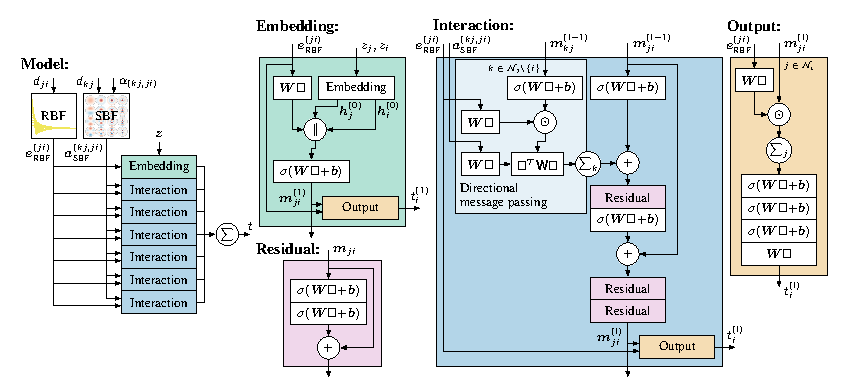
\includegraphics[width=0.78\textwidth]{atomic_simulations/dimenet.pdf}
    \end{figure}
\end{frame}

\begin{frame}{GemNet \footfullcite{https://doi.org/10.48550/arxiv.2106.08903}}
    \centering
    Force- or energy-centric with 3- or 4-way interactions
    \begin{figure}[H]
        \vspace*{-1em}
        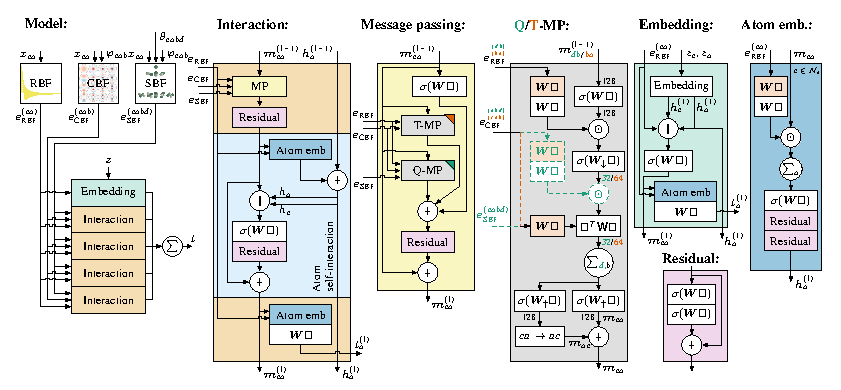
\includegraphics[width=0.82\textwidth]{atomic_simulations/gemnet.pdf}
    \end{figure}
\end{frame}

\begin{frame}{Open Catalyst Project\footnote{\url{https://opencatalystproject.org/}}}
    \begin{figure}
        \begin{subfigure}[t]{0.49\textwidth}
            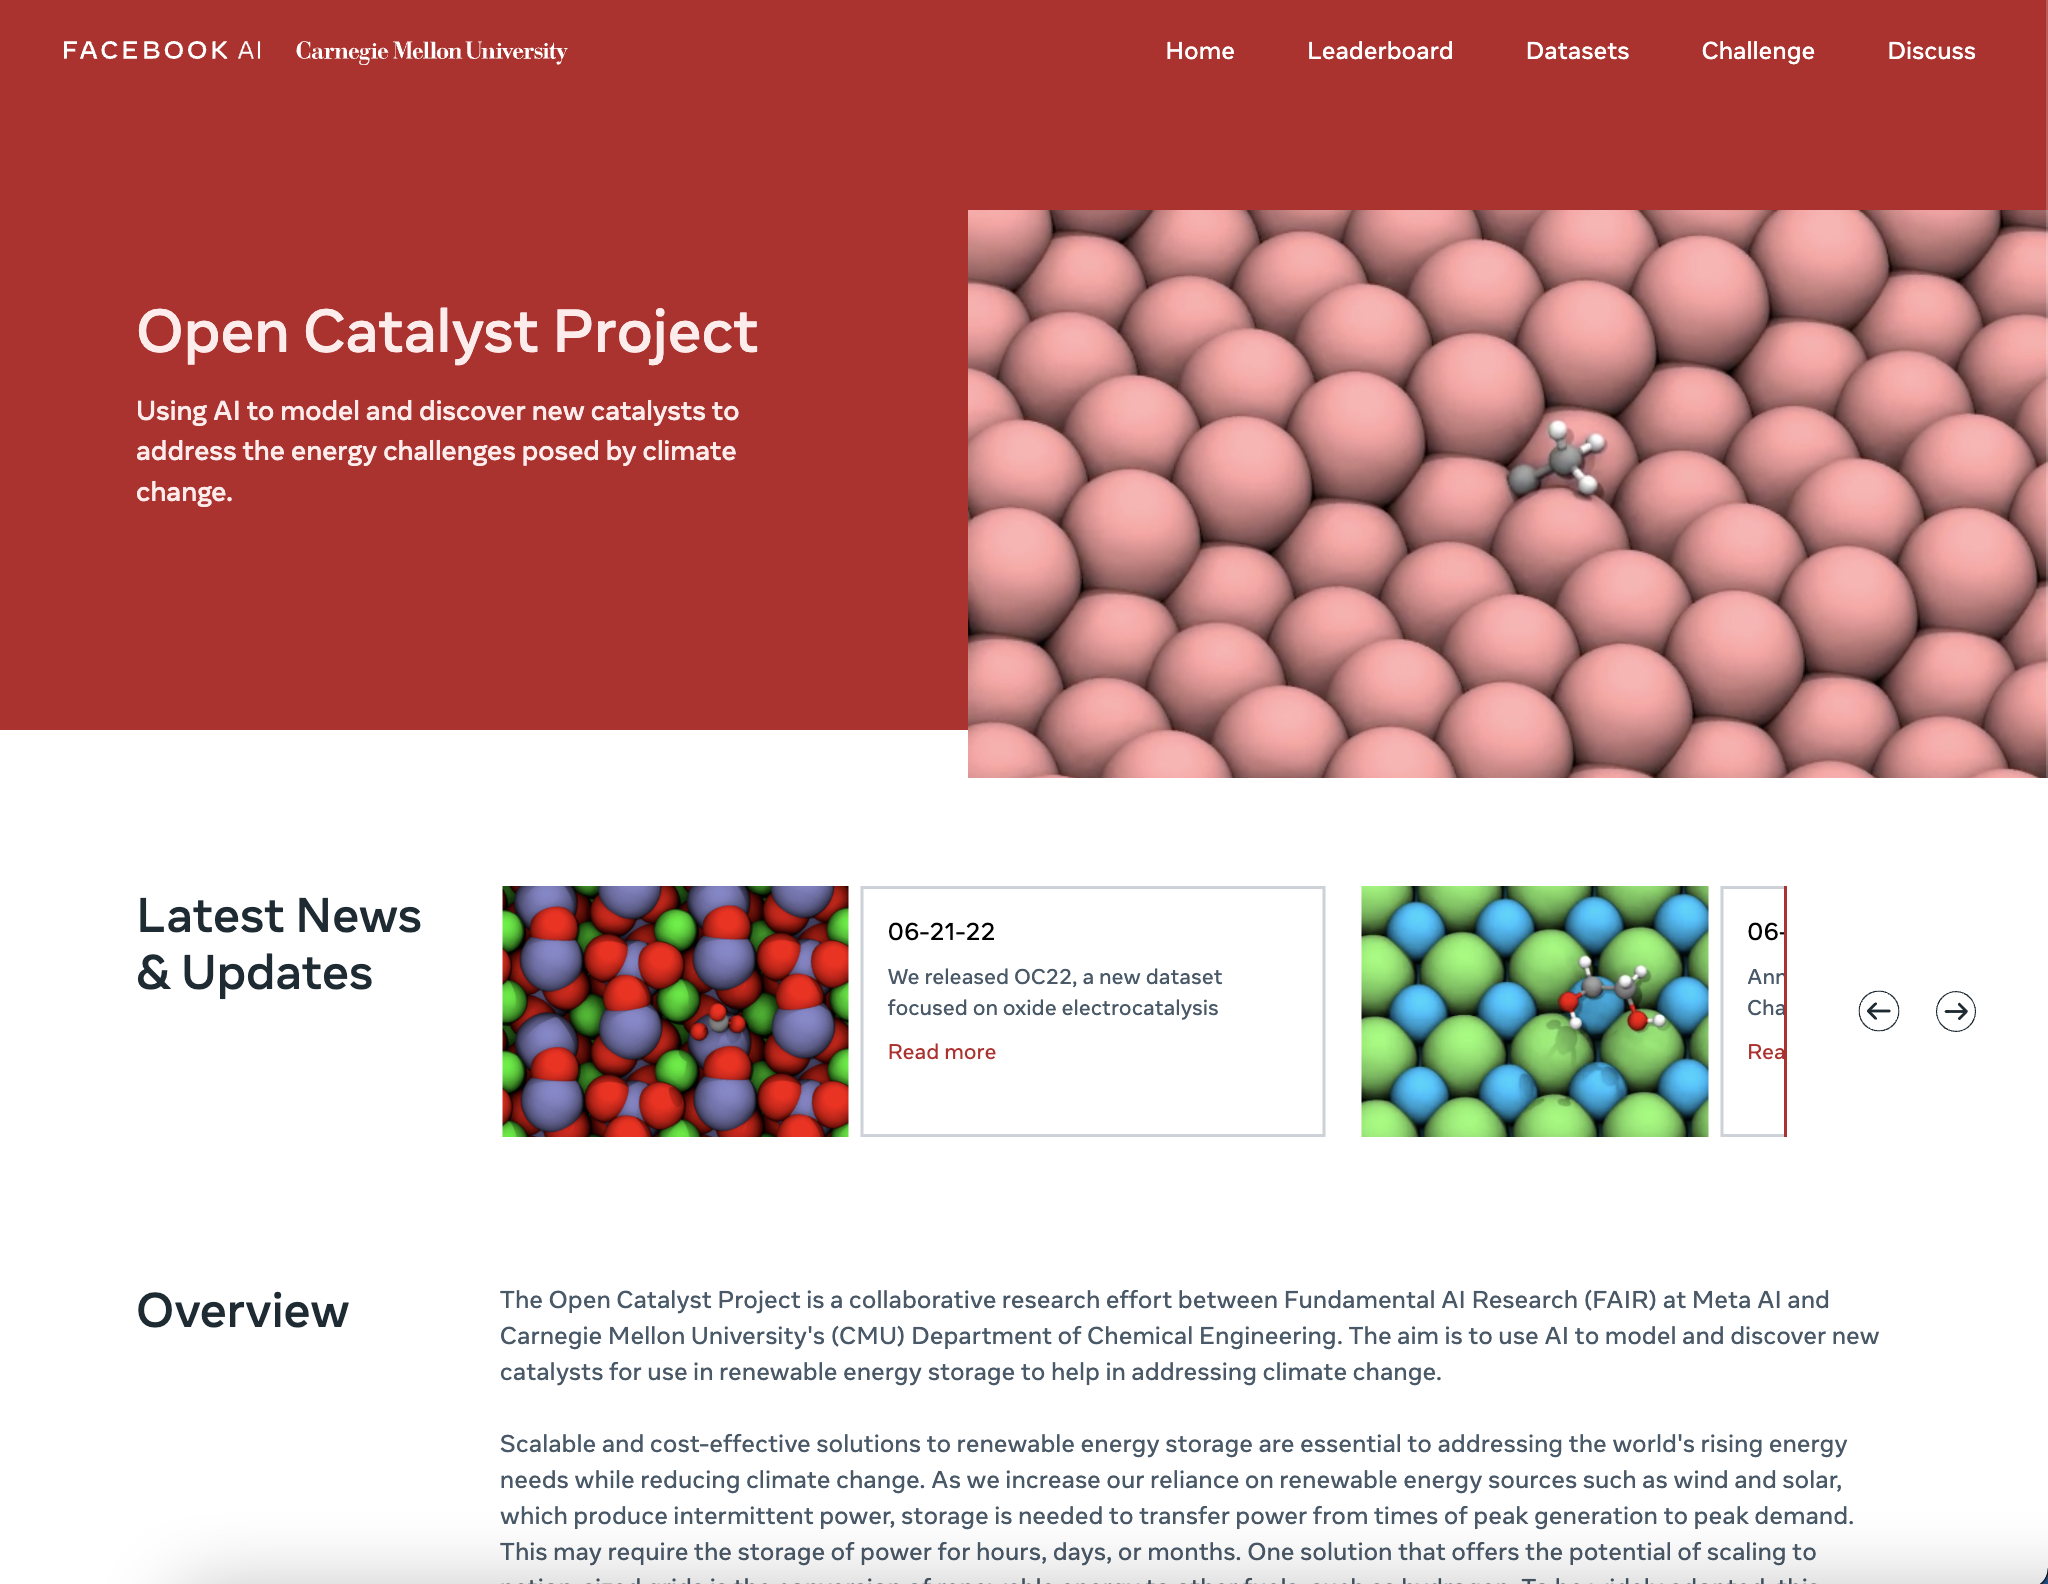
\includegraphics[width=\textwidth]{ocp/OCP.png}
        \end{subfigure}%
        ~
        \begin{subfigure}[t]{0.49\textwidth}
            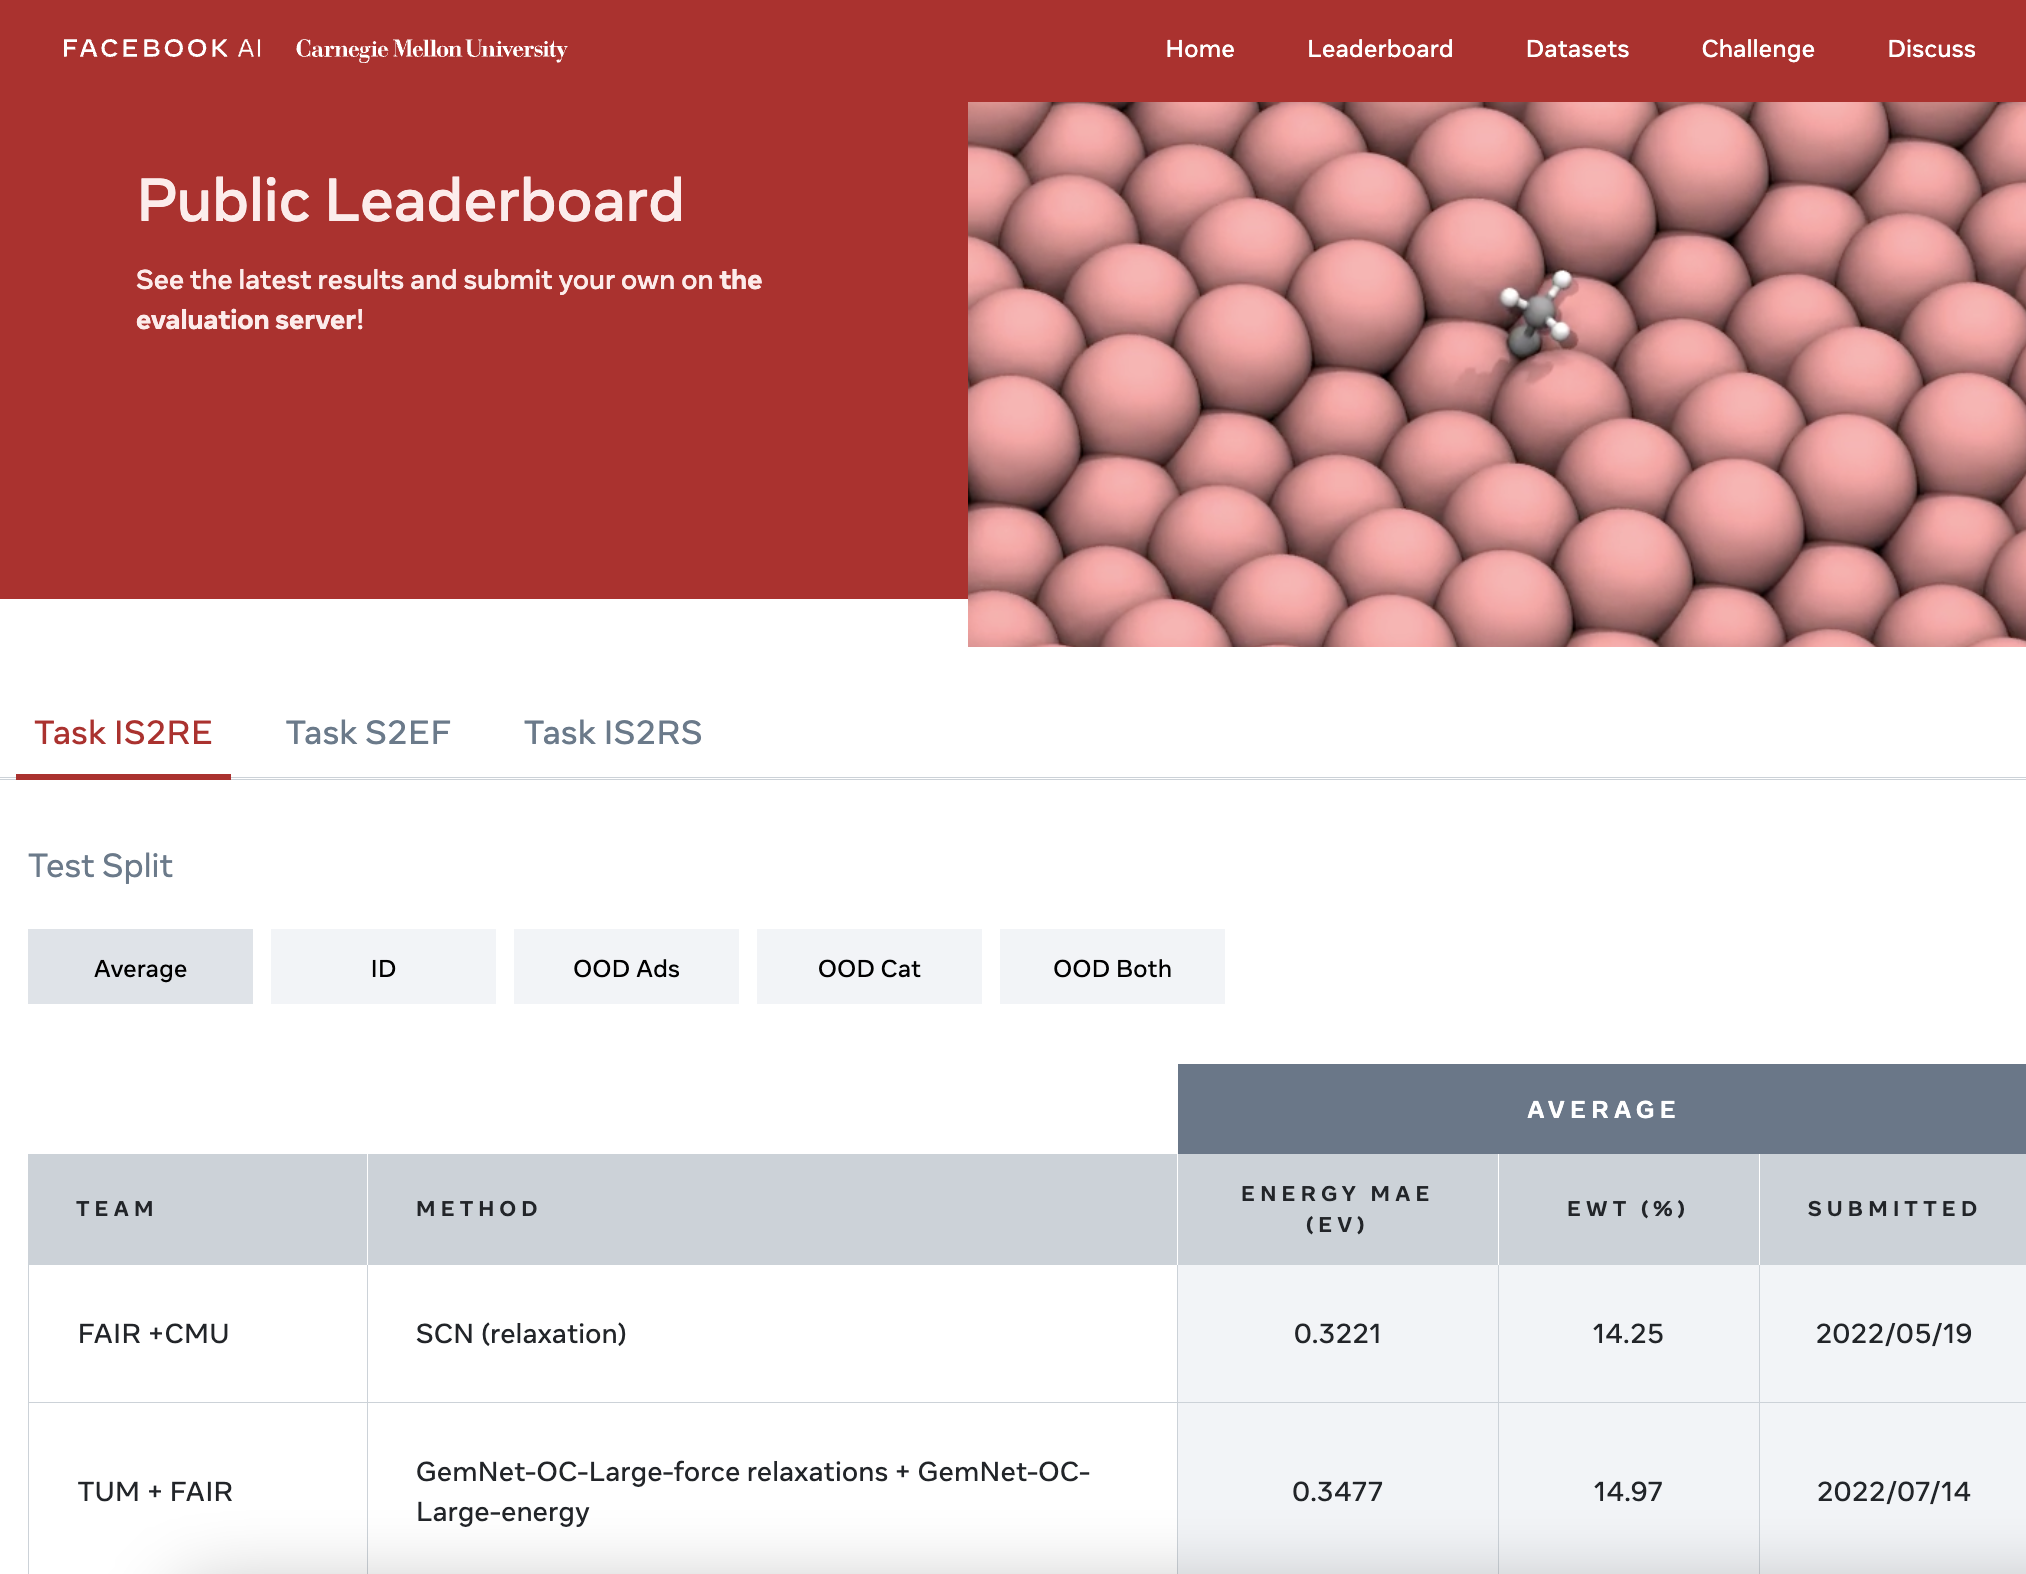
\includegraphics[width=\textwidth]{ocp/OCP_Leaderboard.png}
        \end{subfigure}
    \end{figure}
    \vspace*{1em}
\end{frame}